
%%%%%%%%%%%%%%%%%%%%%%%%%%%%% Define Article %%%%%%%%%%%%%%%%%%%%%%%%%%%%%%%%%%
\documentclass[conference]{IEEEtran}
%%%%%%%%%%%%%%%%%%%%%%%%%%%%%%%%%%%%%%%%%%%%%%%%%%%%%%%%%%%%%%%%%%%%%%%%%%%%%%%

%%%%%%%%%%%%%%%%%%%%%%%%%%%%% Using Packages %%%%%%%%%%%%%%%%%%%%%%%%%%%%%%%%%%
\usepackage{geometry}
\usepackage{graphicx}
\usepackage{amssymb}
\usepackage{amsmath}
\usepackage{amsthm}
    
\usepackage{empheq}
\usepackage{mdframed}
\usepackage{booktabs}
\usepackage{lipsum}
\usepackage{graphicx}
\usepackage{color}
\usepackage{psfrag}
\usepackage{pgfplots}
\usepackage{bm}
\usepackage[spanish]{babel}
\usepackage[utf8]{inputenc} % Codificación UTF-8
\usepackage{amsmath}        % Soporte para ecuaciones matemáticas
\usepackage{graphicx}       % Manejo de imágenes
\usepackage{hyperref}       % Hipervínculos
\usepackage{caption}        % Formato para figuras
\usepackage{multirow}
\usepackage{subcaption}
\usepackage{biblatex}
\usepackage{csquotes}
\usepackage{bookmark}
%%%%%%%%%%%%%%%%%%%%%%%%%%%%%%%%%%%%%%%%%%%%%%%%%%%%%%%%%%%%%%%%%%%%%%%%%%%%%%%

% Other Settings

%%%%%%%%%%%%%%%%%%%%%%%%%% Page Setting %%%%%%%%%%%%%%%%%%%%%%%%%%%%%%%%%%%%%%%
\geometry{a4paper, margin=1in}

%%%%%%%%%%%%%%%%%%%%%%%%%% Define some useful colors %%%%%%%%%%%%%%%%%%%%%%%%%%
\definecolor{ocre}{RGB}{243,102,25}
\definecolor{mygray}{RGB}{243,243,244}
\definecolor{deepGreen}{RGB}{26,111,0}
\definecolor{shallowGreen}{RGB}{235,255,255}
\definecolor{deepBlue}{RGB}{61,124,222}
\definecolor{shallowBlue}{RGB}{235,249,255}
%%%%%%%%%%%%%%%%%%%%%%%%%%%%%%%%%%%%%%%%%%%%%%%%%%%%%%%%%%%%%%%%%%%%%%%%%%%%%%%

%%%%%%%%%%%%%%%%%%%%%%%%%% Define an orangebox command %%%%%%%%%%%%%%%%%%%%%%%%
\newcommand\orangebox[1]{\fcolorbox{ocre}{mygray}{\hspace{1em}#1\hspace{1em}}}
%%%%%%%%%%%%%%%%%%%%%%%%%%%%%%%%%%%%%%%%%%%%%%%%%%%%%%%%%%%%%%%%%%%%%%%%%%%%%%%

%%%%%%%%%%%%%%%%%%%%%%%%%%%% English Environments %%%%%%%%%%%%%%%%%%%%%%%%%%%%%
\newtheoremstyle{mytheoremstyle}{3pt}{3pt}{\normalfont}{0cm}{\rmfamily\bfseries}{}{1em}{{\color{black}\thmname{#1}~\thmnumber{#2}}\thmnote{\,--\,#3}}
\newtheoremstyle{myproblemstyle}{3pt}{3pt}{\normalfont}{0cm}{\rmfamily\bfseries}{}{1em}{{\color{black}\thmname{#1}~\thmnumber{#2}}\thmnote{\,--\,#3}}
\theoremstyle{mytheoremstyle}
\newmdtheoremenv[linewidth=1pt,backgroundcolor=shallowGreen,linecolor=deepGreen,leftmargin=0pt,innerleftmargin=20pt,innerrightmargin=20pt,]{theorem}{Theorem}[section]
\theoremstyle{mytheoremstyle}
\newmdtheoremenv[linewidth=1pt,backgroundcolor=shallowBlue,linecolor=deepBlue,leftmargin=0pt,innerleftmargin=20pt,innerrightmargin=20pt,]{definition}{Definition}[section]
\theoremstyle{myproblemstyle}
\newmdtheoremenv[linecolor=black,leftmargin=0pt,innerleftmargin=10pt,innerrightmargin=10pt,]{problem}{Problem}[section]
%%%%%%%%%%%%%%%%%%%%%%%%%%%%%%%%%%%%%%%%%%%%%%%%%%%%%%%%%%%%%%%%%%%%%%%%%%%%%%%

%%%%%%%%%%%%%%%%%%%%%%%%%%%%%%% Plotting Settings %%%%%%%%%%%%%%%%%%%%%%%%%%%%%
\usepgfplotslibrary{colorbrewer}
\pgfplotsset{width=8cm,compat=1.9}
%%%%%%%%%%%%%%%%%%%%%%%%%%%%%%%%%%%%%%%%%%%%%%%%%%%%%%%%%%%%%%%%%%%%%%%%%%%%%%%

%%%%%%%%%%%%%%%%%%%%%%%%%%%%%%% Title & Author %%%%%%%%%%%%%%%%%%%%%%%%%%%%%%%%
\author{\IEEEauthorblockN{Carlos Fernando Torres Ferrer, Daniel Fernando Aranda Contreras, Dairo Alexander Lobo Moreno,\\ Yulieth Valentina Portilla Jaimes}
\IEEEauthorblockA{Escuela E3T, Universidad Industrial de Santander\\
Correo electrónico: \{carlos2221116, daniel2221648, dairo2221123, yulieth2221136\}@correo.uis.edu.co}}
%%%%%%%%%%%%%%%%%%%%%%%%%%%%%%%%%%%%%%%%%%%%%%%%%%%%%%%%%%%%%%%%%%%%%%%%%%%%%%%
\begin{document}
% Título
\title{\uppercase{Diseño de infraestructura eléctrica de la nueva subestación Huila 230 kV y líneas de transmisión asociadas}}
\maketitle
% Resumen
% Palabras clave        
\begin{IEEEkeywords}
    Nueva subestación Huila, subestación, sistema eléctrico, línea de transmisión, conductores, aislamiento, tensión nomimnal, Neiva.
\end{IEEEkeywords}
\section*{Resumen}
El proyecto UPME 01 - 2022 de la construcción de la subestación Huila 230 y la reconfiguración de las líneas de transmisión mejorará la calidad y la confiabilidad del servicio para fortalecer el sistema eléctrico en la región, reducir las fallas y garantizar que más personas, hogares y actividades productivas tengan acceso a energía segura y continua. Además, este avance es una oportunidad para acompañar el desarrollo económico y social del área, lo que permite que los nuevos sectores y proyectos se conecten con el sistema. 

\section*{Introducción}
En el marco del desarrollo del proyecto para la nueva Subestación Huila 230 kV y sus líneas de transmisión asociadas, este segundo avance se enfoca en el análisis y aplicación de los criterios técnicos de diseño establecidos en la convocatoria y en la normativa vigente del sector eléctrico colombiano. El objetivo principal es asegurar que las soluciones propuestas cumplan con los estándares de calidad, seguridad y eficiencia exigidos para garantizar una operación confiable del sistema. \newline Este avance incluye la revisión de parámetros clave para el diseño eléctrico de la línea de transmisión, así como la definición preliminar del trazado más adecuado, teniendo en cuenta factores técnicos, ambientales y geográficos. Además, se exploran diferentes configuraciones del circuito con el fin de identificar la opción más conveniente tanto desde el punto de vista técnico como económico.
\section{Introducción}
En esta segunda etapa del proyecto de diseño, construcción y puesta en servicio de la nueva subestación Huila 230 kV y sus líneas de transmisión asociadas, se abordan con mayor profundidad los criterios técnicos de diseño exigidos en la convocatoria pública. Este avance se enfoca en el análisis detallado de las especificaciones contenidas en el Anexo 1 de la convocatoria de la UPME, complementadas con los lineamientos establecidos en el Código de Redes (Resolución CREG 025 de 1995 y CREG 098 de 2000), el Reglamento Técnico de Instalaciones Eléctricas (RETIE) y las disposiciones ambientales aplicables.\\ Se revisaron parámetros clave como la potencia nominal en el lado receptor, la capacidad de corriente del circuito, la resistencia DC por fase, los niveles máximos de radio-interferencia y ruido audible, la regulación de tensión, el límite térmico, el tipo de conductor permitido y las condiciones para evitar el efecto corona. Adicionalmente, se evaluaron distintas configuraciones de diseño eléctrico que incluyeron opciones de circuito sencillo y doble circuito con conductores en haz, dispuestos horizontalmente o en triángulo, con separación de 45,72 cm. Se compararon también diferentes tipos de torre y combinaciones de conductores, a fin de asegurar la viabilidad técnica y económica de la solución seleccionada. La configuración final fue escogida con base en su cumplimiento con los parámetros normativos y su conveniencia desde el punto de vista operativo y económico. Finalmente, se calcularon y organizaron en tablas las condiciones eléctricas de operación en ambos extremos de la línea (emisor y receptor), incluyendo datos relevantes como el SIL, la potencia natural, la regulación de tensión, las pérdidas de potencia y demás variables que respaldan la selección técnica.\\ En base a los lineamientos técnicos es posible asegurar que las soluciones propuestas cumplan con los estándares de cálidad, seguridad y eficiencia exigidos para garantizar una operación confiable del sistema. \\Además, se presenta el análisis del trazado propuesto de la línea, identificando la ruta óptima mediante herramientas geográficas como Google Earth, y considerando criterios técnicos, ambientales y topográficos. 




\section{PARÁMETROS DE DISEÑO Y SELECCIÓN DE LA RUTA}

Para la contrucción de la línea de transmisión Huila 230 kV se tomaron en cuenta espeficicaciones y criterios técnicos de diseño basados en el RETIE, CREG y la UPME. Contemplando una potencia nóminal de 700 MVA y un factor de potencia de 0.9 en atraso, se cálcula la corriente en el lado receptor que da un valor de 1757 [A]. Para la elección de conductor es muy importante analizar la capacidad de corriente de operación del circuito para evitar que el conductor se sobrecaliente o se dañe, en este caso, se toma una mayor a 2400 amperios a temperatura ambiente máxima promedio y se toma resistencia DC a 20 grados Celsius como 0,0230 ohmios/km.\\
Uno de los efectos de gran importancia en líneas de transmisión (LT) es el efecto corona, este es un fenómeno eléctrico causado por la ionización del aire circundante a los conductores eléctricos debido a la colisión de electrones libres que se escapan del sistema. En el momento que las moléculas de aire se ionizan, éstas son capaces de conducir la corriente eléctrica y parte de los electrones que circulan por la línea pasan a circular por el aire. Cuando ocurre el Efecto Corona este crea ozono, el ozono deteriora material dieléctrico con base de goma y/o plástico; si existen condiciones de humedad el ozono puede crear ácido nítrico que es capaz de atacar al cobre y otros metales causando corrosión, por tanto en la construcción de la línea no se deberá presentar efecto corona en condiciones de buen tiempo; y es a raíz de este que se desarrollan fenómenos tales como la radio interferencia (degradación de una señal de radio que perturba la recepción de radio, televisión, teléfonos inalámbricos y otros dispositivos) y el ruido audible (zumbido), los cuales con el aumento de la tensión de operación se hacen cada vez más notorios, y aumentan así la posibilidad de que tanto personas como equipos puedan ser afectados o interferidos debido a las propiedades electromagnéticas que se generan en los alrededores de la LT. Por eso todos los equipos y conectores deberán ser contruidos cumpliendo a una relación señal-ruido mínima de: a) Zona Rurales: 22 dB a 80m del eje de la línea a 1000 kHz en condiciones de buen tiempo y b) Zonas Urbanas: 22 dB a 40m del eje de la línea a 1000 kHz en condiciones de buen tiempo y en cuanto a ruido audible generado por la línea y/o la subestación, deberá limitarse a los estándares máximos permisibles de niveles de emisión de ruido establecidos en Resolución 0627 de 2006 (abril 7) Ministerio de Ambiente y Desarrollo Sostenible.\\
Para la correcta elección del conductor, también se consideró el cumplimiento de la regulación de tensión, que debe estar dentro del rango permitido de ±10 \%. Además, se verificó el límite térmico, asegurando que la temperatura del conductor bajo condiciones normales de operación no supere los 75 °C. Las pérdidas por efecto Joule también se controlaron, garantizando que no excedan el 3 \% por cada 100 km de línea, tomando como base la resistencia del conductor a 75 °C.\\
Como parte del diseño del sistema de transmisión a 230 kV en el departamento del Huila, se planteó inicialmente una interconexión eléctrica entre tres subestaciones: Subestación Betania, Nueva Subestación Huila y Subestación Tuluní. Para ello, se realizó una evaluación general del territorio utilizando la herramienta Google Earth Pro, lo cual permitió identificar un trazado preliminar que conecta las tres subestaciones, evaluando condiciones topográficas, uso del suelo, áreas sensibles, cuerpos de agua y cercanía a centros poblados.\\
La ruta general del proyecto tiene una longitud aproximada de 160,45 km, atravesando principalmente zonas rurales, con tramos de topografía montañosa y presencia agrícola. Esta visión integral sirvió como base para la planeación técnica y estratégica del sistema de transmisión.\\

\begin{figure}[!ht]
\centering
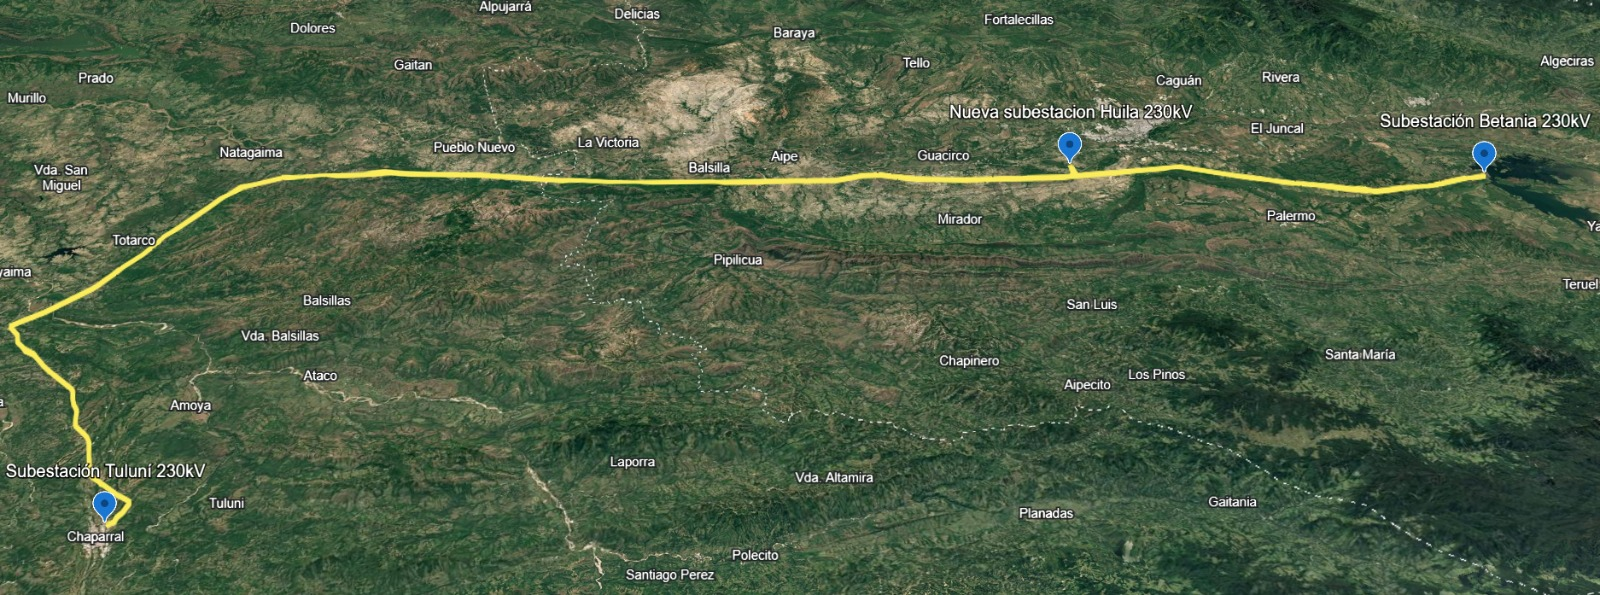
\includegraphics[width=1\linewidth]{img/Trazado.jpg}
\caption{Trazado general del sistema con Google Earth.}
\label{fig:general}
\end{figure}
Si bien el proyecto contempla un sistema de mayor longitud, el análisis técnico y eléctrico detallado se centró exclusivamente en el tramo comprendido entre la Subestación Betania y la Nueva Subestación Huila, con una longitud aproximada de 31 km. Este segmento fue seleccionado por presentar condiciones topográficas representativas del recorrido general, y por su relevancia estratégica en la primera fase del proyecto.

Para este tramo se realizó un trazado más preciso utilizando también Google Earth Pro, lo cual permitió identificar una ruta técnicamente viable que evita interferencias con zonas urbanas o áreas de protección ambiental. El entorno geográfico cercano a la nueva subestación Huila fue evaluado en detalle, considerando aspectos como accesibilidad, pendientes y cercanía a corredores de infraestructura existentes. Este tramo fue tomado como referencia para el cálculo de parámetros eléctricos, estudios de diseño geométrico y evaluación de fenómenos como el efecto corona, dada su representatividad y factibilidad técnica dentro del sistema propuesto.

\begin{figure}[!ht]
\centering
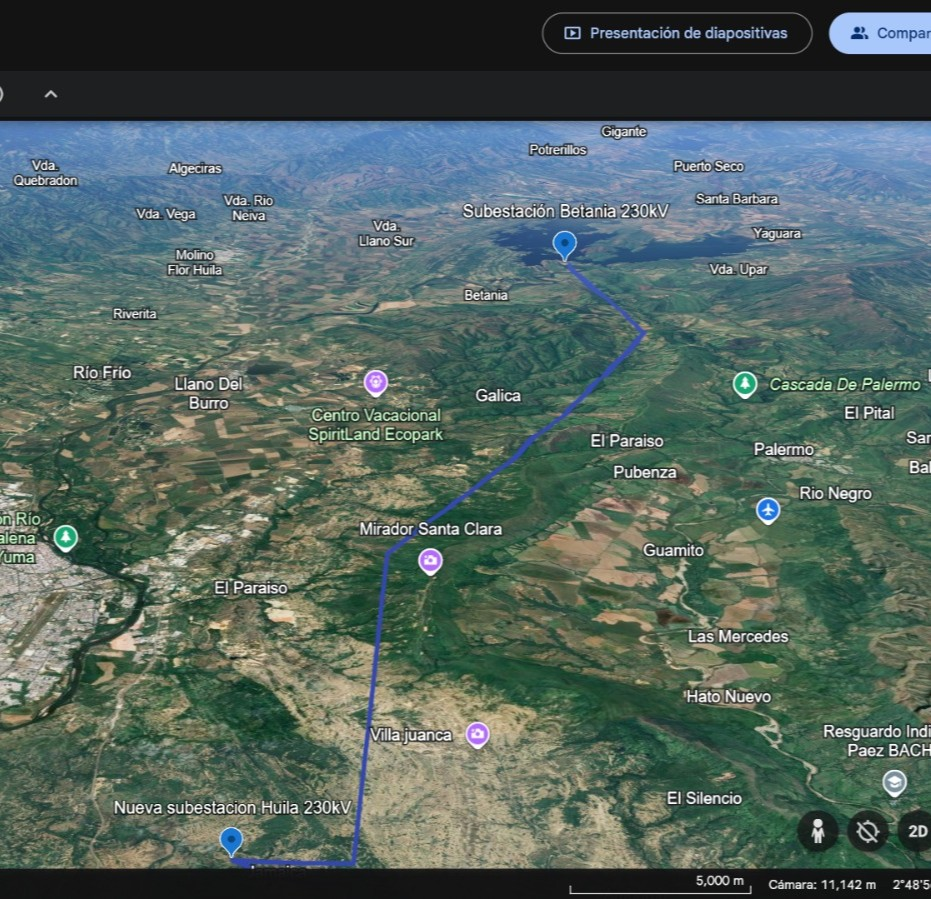
\includegraphics[width=0.48\linewidth]{img/conexion.jpg}
\caption{Trazado Línea Betania - Huila.}
\label{fig:tramoBH}
\end{figure}

Este tramo fue tomado como referencia para el cálculo de parámetros eléctricos, estudios de diseño geométrico, modelado de cargas, y evaluación de fenómenos como el efecto corona, dada su representatividad y factibilidad técnica dentro del sistema propuesto.

\section*{Criterios de selección del trazado y evaluación de alternativas}

Para la selección del trazado se evaluaron distintos criterios técnicos, geográficos y ambientales que permitieran definir el recorrido más adecuado. A continuación, se resumen los aspectos más relevantes:

\begin{itemize}
    \item Se priorizó el paso por zonas con pendientes moderadas y buena accesibilidad, lo que facilita tanto la construcción como el mantenimiento futuro de la línea.
    
    \item Se evitó que el trazado atravesara áreas urbanas, centros poblados o zonas densamente habitadas, con el fin de reducir afectaciones sociales y costos asociados a servidumbres.
    
    \item Se buscó mantener una distancia prudente con áreas protegidas, zonas de valor ambiental o ecosistemas frágiles (como ríos y quebradas), para minimizar afectaciones y garantizar la estabilidad de las estructuras.
    
    \item Se procuró mantener el trazado cercano a vías ya existentes, lo cual facilita el transporte de materiales y el acceso para la construcción de torres.
    
    \item En cuanto a las alternativas de trazado, se evaluaron varias rutas con diferentes configuraciones y longitudes. Algunas opciones implicaban atravesar terrenos montañosos o con vegetación densa, lo que incrementaba la complejidad técnica y los costos de construcción. Otras alternativas ofrecían trayectos más accesibles, pero con mayor longitud total, lo que incrementaba las pérdidas eléctricas y los costos de operación.
\end{itemize}


Finalmente, la ruta seleccionada fue aquella que representó un equilibrio entre viabilidad técnica, facilidad de acceso, menor afectación ambiental y cercanía a infraestructuras existentes, como vías y caminos rurales. Esta decisión se apoyó tanto en el análisis geoespacial como en criterios de diseño 
eléctrico, buscando garantizar la confiabilidad del sistema y el cumplimiento de la normativa vigente.
\section{Elección del conductor: Flint (AAAC)}

En el diseño de la línea de transmisión asociada a la nueva subestación Huila 230 kV, se consideraron diferentes tipos de conductores con base en criterios eléctricos, mecánicos y ambientales. Las opciones evaluadas fueron AAC (Aluminium Conductor, All), ACAR (Aluminium Conductor Alloy Reinforced) y AAAC (All Aluminium Alloy Conductor). Tras el análisis, se seleccionó el conductor Flint, de tipo AAAC, por ser el que mejor se adapta a los requerimientos técnicos del proyecto y a las condiciones climáticas de la región. \\ El departamento del Huila presenta un clima predominantemente cálido, con temperaturas medias superiores a 25 °C y una humedad relativa considerable en varias zonas. Estas condiciones pueden acelerar procesos de corrosión, especialmente en conductores con componentes ferrosos o poco resistentes a ambientes húmedos.
El conductor \textbf{Flint (AAAC)} fue seleccionado por las siguientes razones:

\begin{itemize}
    \item \textbf{Mejor desempeño frente al AAC:} Aunque el AAC tiene excelente conductividad eléctrica, su resistencia mecánica es considerablemente menor, lo que implica estructuras de soporte más robustas y costosas. Además, el AAC es más susceptible a la corrosión en ambientes húmedos, por lo que no es ideal para una zona como el Huila.
    
    \item \textbf{Mayor resistencia mecánica y menor peso:} En comparación con el ACAR, que incluye un núcleo de acero, el AAAC ofrece buena resistencia mecánica sin aumentar el peso significativamente. Esto facilita el diseño de estructuras más ligeras y económicas.
    
    \item \textbf{Resistencia a la corrosión:} Al estar compuesto por una aleación de aluminio resistente, el AAAC ofrece una durabilidad superior en zonas con alta humedad, evitando problemas de oxidación comunes en conductores con núcleo de acero.
    
    \item \textbf{Baja resistencia eléctrica (Rdc):} El conductor Flint presenta una baja resistencia en corriente continua, lo cual reduce las pérdidas por efecto Joule y mejora la eficiencia energética de la línea.
    
    \item \textbf{Compatibilidad con ambientes cálidos:} La aleación del AAAC mantiene su desempeño incluso a temperaturas elevadas, permitiendo una operación confiable en condiciones térmicas exigentes como las del Huila.
\end{itemize}

En resumen, el conductor Flint (AAAC) se eligió por su excelente equilibrio entre eficiencia eléctrica, resistencia mecánica y comportamiento frente a la corrosión. Frente al AAC, que aunque es más económico inicialmente, presenta limitaciones importantes en durabilidad y requerimientos estructurales, y frente al ACAR, que es más pesado y más costoso de instalar, el AAAC se posiciona como la alternativa más adecuada para las condiciones técnicas y ambientales del proyecto en el Huila.
\subsection{Calculos circuito simple en dispociosición triangulo para haz de un solo conductor}

\begin{figure}[ht!]
    \centering
    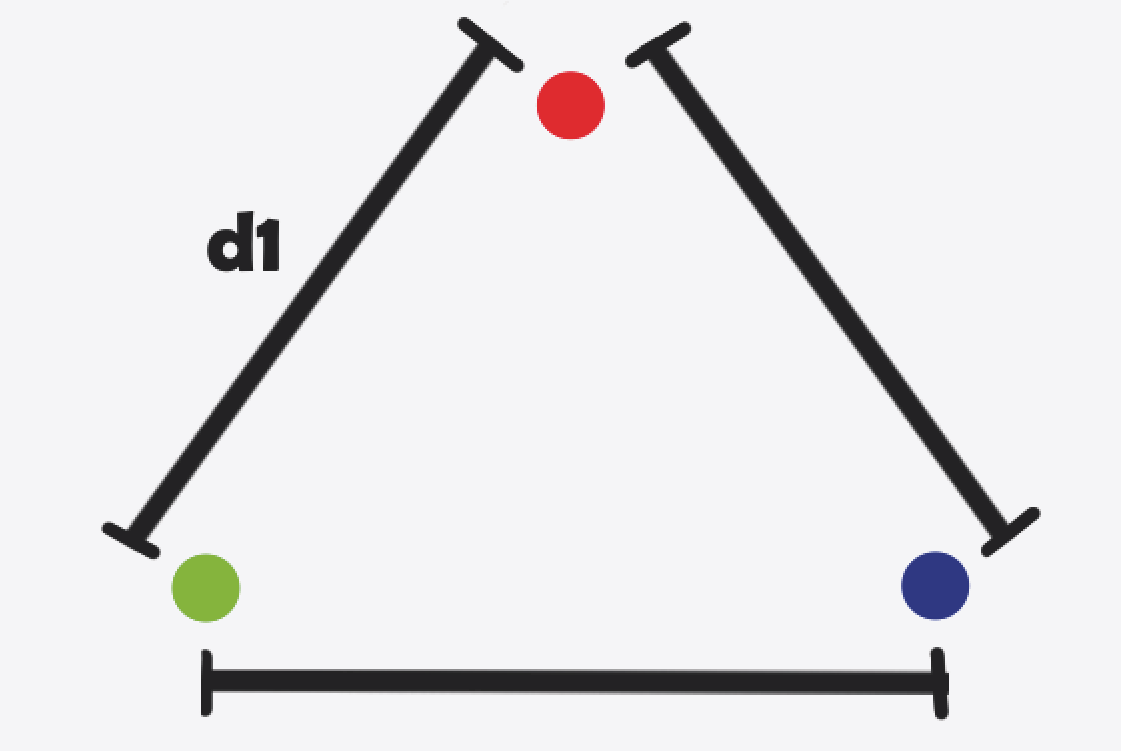
\includegraphics[width=0.48\textwidth]{img/Calculos circuito simple en dispociosición triangulo para haz de un solo conductor disp.png}
    \caption{circuito simple con fases en dispociosición triangulo para haz de un solo conductor.}
    \label{fig:circuito_simple_disp}
\end{figure}

\begin{figure}[ht!]
    \centering
    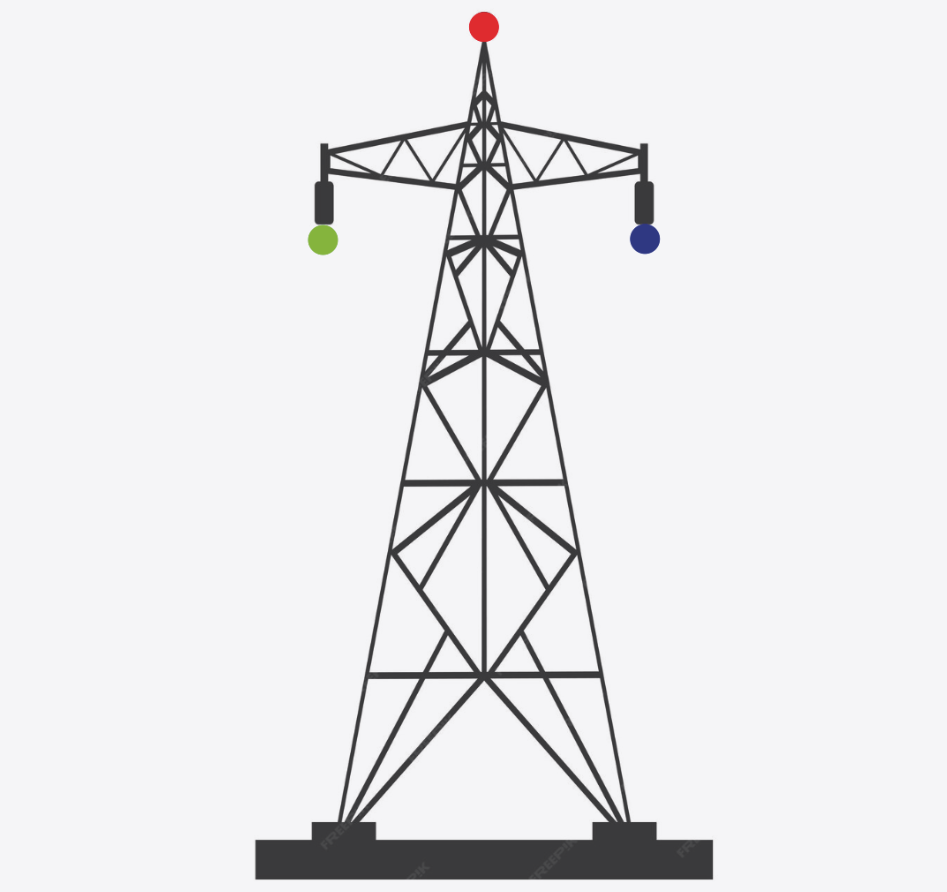
\includegraphics[width=0.48\textwidth]{img/Calculos circuito simple en dispociosición triangulo para haz de un solo conductor.png}
    \caption{circuito simple con fases en dispociosición triangulo para haz de un solo conductor.}
    \label{fig:circuito_simple_Torre}
\end{figure}



\textbf{Datos del conductor: Flint 746,4 kcmil}
\begin{itemize}
  \item Longitud línea: $l = 31 \, \text{km}$
  \item Temperatura: $T = 28^\circ$C
  \item $s = 0.4572$ [m]
  \item Radio: $r = 12.58$ [mm]
  \item $f = 60$ [Hz]
  \item RMG = 9.66 [cm]
  \item Resistencia a 75°C: $R_{75} = 0.106 \, \Omega/\text{km}$
  \item $\alpha_0$ aluminio = 0.00438
\end{itemize}

\vspace{0.5cm}

\subsection*{Cálculo de Resistencia equivalente por fase:}

\[
R_{28} = \left( \frac{1 + \alpha_0 \cdot28}{1 + \alpha_0 \cdot 75} \right) \cdot R_{75} = 0.0895488 \, \frac{\Omega}{\text{km}}
\]

\[
R_{\text{eq}} = 0.0895488 \, \frac{\Omega}{\text{km}} = 0.0895488 \cdot 31 = 2.7768 \, [\Omega]
\]

\vspace{0.5cm}
\subsection*{Cálculo de Reactancia Inductiva:}


\[
DMG_{e} = \sqrt[3]{d1 \cdot d1 \cdot d1} = 12 \, [\text{m}]
\]

\vspace{0.3cm}
\[
RMG_{e} = radio\cdot e^{(-1/4)} = 9.7973 \, [\text{mm}]
\]

\vspace{0.3cm}
\[
X_L = 31\cdot 2\pi \cdot f \cdot2\cdot 10^{-4} \cdot \ln\left( \frac{DM_{Ge}}{RMG_e} \right) = 16.6198\, [\Omega]
\]

\[
z_T = \left[ R_{\text{eq}T} + jX_L \right] = 2.7768 + j16.6198 \quad [\Omega]
\]

\subsection*{Cálculo de la capacitancia:}

\[
RMG_{e} = radio = 12.58 \, [\text{mm}]
\]

\[
C_T = \left[ 31 \cdot \left(18 \cdot 10^9 \cdot \ln\left( \frac{DMG_e}{RMG_e} \right) \right)^{-1} \right]
\]

\[
C_T =  242.2065 \, [nF]
\]


\[
Y_T = j\cdot2\pi \cdot f \cdot C_T = j91.309 \, [\mu S]
\]

\section*{Parámetros de la línea y receptor:}

\begin{align*}
A &= 1 + \frac{Z_T \cdot Y_T}{2} = 0.9992 + j\,1.2677 \times 10^{-4} \\
B &= Z_T = 2.7768 +16.6198i \quad [\Omega] \\
C &= Y_T \left(1 + \frac{Z_T \cdot Y_T}{4} \right) \\
C &= C = -5.7879e-09 + 9.1275e-05i \quad [S] \\
D &= A =  0.9992 + j\,1.2677 \times 10^{-4} 
\end{align*}

\begin{align*}
I_R &= \frac{S}{\sqrt{3} \cdot V_L} \cdot \angle -\cos(\text{fp})  \\
I_R &= 1757.15299 \angle  -25.84193 ^\circ \quad [A] \\
V_R &= \frac{V_L}{\sqrt{3}} \angle 0^\circ = 132.79056 \angle 0^\circ \quad [kV]
\end{align*}

\section*{Parámetros del Generador}

\begin{align*}
V_G &= A \cdot V_R + B \cdot I_R \\
I_G &= B \cdot V_R + D \cdot I_R
\end{align*}

\begin{align*}
V_G &= 151.7484 \angle 9.16614^\circ \quad [kV] \\
I_G &= 1750.5712 \angle -25.477^\circ \quad [A]
\end{align*}

\[
\%RV = \left( \frac{ |V_G| }{ |A| \cdot |V_R| } \right) - 1 = 14.3633\%
\]
\[
\% \text{Pérdida} = 100*\frac{P_g - P_r}{P_g} =  3.9113\%
\]
\[
\% \eta =100* \frac{P_r}{P_g} = 96.0887\%
\]

\section*{Efecto Corona}

\begin{align*}
m_c &= 0{,}95 \\
m_t &= 1 \\
r &= 400 \quad [\text{m}] \\
T &= 28^\circ \text{C}
\end{align*}

\begin{align*}
h &= 10^{\log_{10}(76) - \frac{y}{18336}} \Rightarrow h = 72.2767 \\
\delta &= \frac{3{,}921 \cdot h}{273 + T} = 0.9410
\end{align*}

\begin{align*}
U_c &= 84 \cdot m_c \cdot m_t \cdot \delta \cdot \log \left( \frac{DMG}{r} \right) \quad [\text{kV}]
\end{align*}

\begin{align*}
U_{ne} &= 1{,}15 \cdot U_{\text{línea}} \quad [\text{kV}]
\end{align*}

\begin{align*}
U_{ne} < U_c &\Rightarrow 264.5 \leq 281.4748 \\
&\text{No se presenta efecto Corona}
\end{align*}
\section*{Circuito doble con haz de 3 Conductores}

\begin{figure}[ht!]
\centering
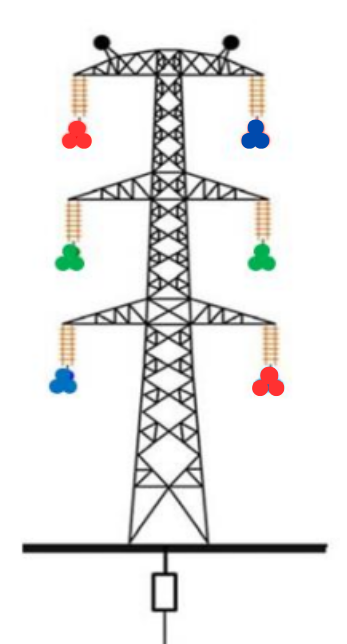
\includegraphics[width=0.48\linewidth]{img/torre3.png}
\caption{Configuración de la torre.}
\label{fig:torre3}
\end{figure}



\begin{figure}[ht!]
\centering
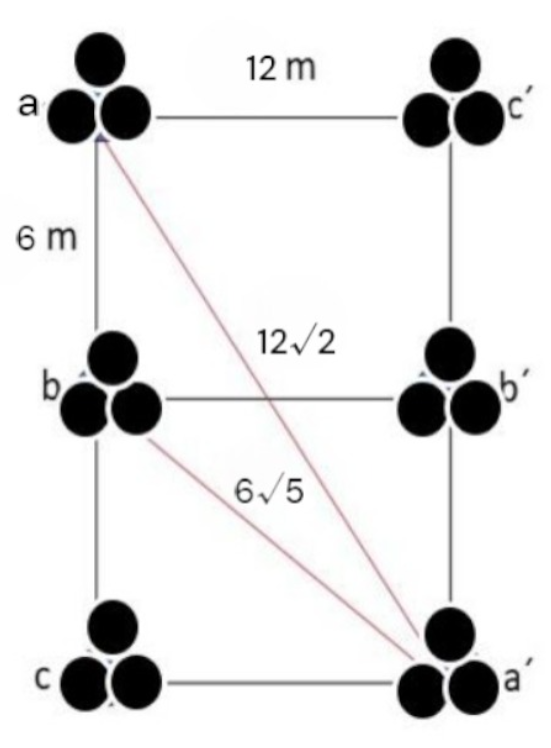
\includegraphics[width=0.48\linewidth]{img/distancia3.png}
\caption{Distancias entre conductores.}
\label{fig:distancia3}
\end{figure}



\textbf{Datos del conductor: Flint 746,4 kcmil}
\begin{itemize}
  \item Longitud línea: $l = 31 \, \text{km}$
  \item Temperatura: $T = 28^\circ$C
  \item $s = 0.4572$ [m]
  \item Radio: $r = 12.58$ [mm]
  \item $f = 60$ [Hz]
  \item RMG = 9.66 [cm]
  \item Resistencia a 75°C: $R_{75} = 0.106 \, \Omega/\text{km}$
  \item $\alpha_0$ aluminio = 0.00438
\end{itemize}

\vspace{0.5cm}

\subsection*{Cálculo de Resistencia equivalente por fase:}

\[
R_{28} = \left( \frac{1 + \alpha_0 \cdot28}{1 + \alpha_0 \cdot 75} \right) \cdot R_{75} = 0.0895488 \, \frac{\Omega}{\text{km}}
\]

\[
R_{\text{eq}} = \frac{l \cdot R_{28}}{6} = \frac{31 \cdot 0.0895488}{6} = 0.4628 \, [\Omega]
\]

\vspace{0.5cm}
\subsection*{Cálculo de Reactancia Inductiva:}

\[
DMG_{AB} = \sqrt[4]{D_{12} \cdot D_{12'} \cdot D_{1'2} \cdot D_{1'2'}} = 8.942 \, [\text{m}]
\]

\[
DMG_{AC} = \sqrt[4]{D_{13} \cdot D_{13'} \cdot D_{1'3} \cdot D_{1'3'}} = 12 \, [\text{m}]
\]

\[
DMG_{BC} = \sqrt[4]{D_{23} \cdot D_{23'} \cdot D_{2'3} \cdot D_{2'3'}} = 8.942 \, [\text{m}]
\]

\[
DMG_{e} = \sqrt[3]{D_{AB} \cdot D_{BC} \cdot D_{CA}} = 9.88524 \, [\text{m}]
\]

\vspace{0.3cm}
\[
RMG_{haz} = \sqrt[3]{RMG \cdot s^2} = 0.2126 \, [\text{m}]
\]

\[
RMG_{a} = \sqrt{RMG_{haz} \cdot D_{11'}} = 1.46457 \, [\text{m}]
\]

\[
RMG_{b} = \sqrt{RMG_{haz} \cdot D_{22'}} = 1.231559 \, [\text{m}]
\]

\[
RMG_{c} = \sqrt{RMG_{haz} \cdot D_{33'}} = 1.46457 \, [\text{m}]
\]

\[
RMG_{e} = \sqrt[3]{RMG_{a} \cdot RMG_{b} \cdot RMG_{c}} = 1.38238 \, [\text{m}]
\]

\vspace{0.3cm}
\[
X_L = 31\cdot 2\pi \cdot f \cdot2\cdot 10^{-4} \cdot \ln\left( \frac{DM_{Ge}}{RMG_e} \right) = 4.54872 \, [\Omega]
\]

\[
z_T = \left[ R_{\text{eq}T} + jX_L \right] = 0,\!4628 + j4,\!5981 \quad [\Omega]
\]

\subsection*{Cálculo de la capacitancia:}

\[
DMG_{e} = \sqrt[3]{D_{AB} \cdot D_{BC} \cdot D_{CA}} = 9.88524 \, [\text{m}]
\]

\[
RMG_{haz} = \sqrt[3]{r \cdot s^2} = \sqrt{0.01258 \cdot 0.4572^2} = 0.138027 \, [\text{m}]
\]

\[
RMG_{a} = \sqrt{RMG_{haz} \cdot D_{11'}} =   1.530489 \, [\text{m}]
\]

\[
RMG_{b} = \sqrt{RMG_{haz} \cdot D_{22'}} = 1.28698 \, [\text{m}]
\]

\[
RMG_{c} = \sqrt{RMG_{haz} \cdot D_{33'}} = 1.530489 \, [\text{m}]
\]

\[
RMG_{e} = \sqrt[3]{RMG_{a} \cdot RMG_{b} \cdot RMG_{c}} = 1.444589 \, [\text{m}]
\]

\[
C_T = \left[ 31 \cdot \left(18 \cdot 10^9 \cdot \ln\left( \frac{DMG_e}{RMG_e} \right) \right)^{-1} \right] = 11.36542 \, [\text{pF}]
\]

\[
Y_T = j\cdot2\pi \cdot f \cdot C_T = j4,\!2846 \times 10^{-9} \quad [\text{S}]
\]

\section*{Parámetros de la línea y receptor:}

\begin{align*}
A &= 1 + \frac{Z_T \cdot Y_T}{2} = 0.9999 + j\,9.911756 \times 10^{-10} \\
B &= Z_T = 0.4628 + j\,4.5981 \quad [\Omega] \\
C &= Y_T \left(1 + \frac{Z_T \cdot Y_T}{4} \right) \\
C &= -2.1241 \times 10^{-18} + j\,4.28466 \times 10^{-9} \quad [S] \\
D &= A = 0.9999 + j\,9.911756 \times 10^{-10}
\end{align*}

\begin{align*}
I_R &= \frac{S}{\sqrt{3} \cdot V_L} \cdot \angle -\cos(\text{fp}) = 1757.15299 \angle -25.844^\circ \quad [A] \\
I_R &= 1757.15299 \angle -25.844^\circ \quad [A] \\
V_R &= \frac{V_L}{\sqrt{3}} \angle 0^\circ = 132.79056 \angle 0^\circ \quad [kV]
\end{align*}

\section*{Parámetros del Generador}

\begin{align*}
V_G &= A \cdot V_R + B \cdot I_R \\
I_G &= B \cdot V_R + D \cdot I_R
\end{align*}

\begin{align*}
V_G &= 137.27837 \angle 2.89^\circ \quad [kV] \\
I_G &= 1757.1574 \angle -25.84478^\circ \quad [A]
\end{align*}

\[
\%RV = \left( \frac{ |V_G| }{ |A| \cdot |V_R| } \right) - 1 = 3{,}33\%
\]
\[
\% \text{Pérdida} = 100*\frac{P_g - P_r}{P_g} = 0{,}6759\%
\]
\[
\% \eta =100* \frac{P_r}{P_g} = 99{,}32\%
\]

\section*{Efecto Corona}

\begin{align*}
m_c &= 0{,}95 \\
m_t &= 1 \\
r &= 400 \quad [\text{m}] \\
T &= 28^\circ \text{C}
\end{align*}

\begin{align*}
h &= 10^{\log_{10}(76) - \frac{y}{18336}} \Rightarrow h = 72.2767 \\
\delta &= \frac{3{,}921 \cdot h}{273 + T} =0.941
\end{align*}

\begin{align*}
U_c &= 84 \cdot m_c \cdot m_t \cdot \delta \cdot \log \left( \frac{DMG}{r} \right) \quad [\text{kV}]
\end{align*}

\begin{align*}
U_{ne} &= 1{,}15 \cdot U_{\text{línea}} \quad [\text{kV}]
\end{align*}

\begin{align*}
U_{ne} < U_c &\Rightarrow 264.5 \leq 273.527 \\
&\text{No se presenta efecto Corona}
\end{align*}
\section{Circuito simple con haz de 3 Conductores}

\begin{figure}[h!]
    \centering
    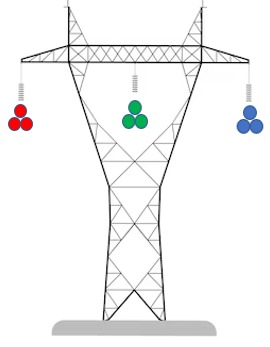
\includegraphics[width=0.48\linewidth]{img/sencillotriplex.jpg}
    \caption{Circuito sencillo 3 conductores disposición horizontal}
    \label{fig:enter-label}
\end{figure}

\begin{figure}[h!]
    \centering
    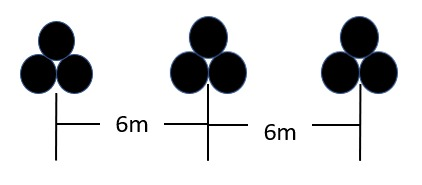
\includegraphics[width=0.48\linewidth]{img/disposicion.jpg}
    \caption{}
    \label{fig:enter-label2}
\end{figure}
\textbf{Datos:}

\begin{align*}
L &= 31~\text{km} & r &= 12,58~\text{mm} \\
S &= 0.4537~[\text{m}] & \alpha_0 &= 0.00438~[\text{mm}] \\
f &= 60~[\text{Hz}] & \text{RMG tabla} &= 9.66~[\text{mm}] \\
R_{\text{AC}75^\circ C} &= 0.106\Omega/\text{km} & V_L &= 230~\text{kV} \\
T_2 &= 28^\circ C & T_1 &= 75^\circ C \\
S &= 700~\text{MVA} & \text{FP} &= 0.9~\text{atraso}
\end{align*}

\begin{align*}
R_{\text{AC}~28^\circ C} &= \left( \frac{1 + \alpha_0 T_2}{1 + \alpha_0 T_1} \right) \cdot R_{\text{75}^\circ C} \\
&= \left( \frac{1 + (0.00438)(28)}{1 + (0.00438)(75)} \right) \cdot 0.106 \\
&= 0.08957~\Omega/\text{km}
\end{align*}

\textbf{Resistencia total por fase:}
\begin{align*}
R_{\text{Fase}} &= \frac{R_{\text{AC}~28^\circ C}}{\text{\#Conductores} \cdot \text{\#Circuitos}} \\
&= \frac{0.08957}{3(1)} = 0.9256~\Omega
\end{align*}

\textbf{Cálculo de la distancia media geométrica:}
\begin{align*}
DMG_{eq} &= \sqrt[3]{D_{12} D_{13} D_{23}} = 7.5595~\text{m}
\end{align*}

\textbf{Radio medio geométrico equivalente de la inductancia:}
\begin{align*}
RMGL_{eq} &= \sqrt[3]{\text{RMG tabla} \cdot S^2} = 0.12639~\text{m}
\end{align*}

\textbf{Inductancia total:}
\begin{align*}
L &= \left(2 \cdot 10^{-4} \right) \ln \left( \frac{DMG_{eq}}{RMGL_{eq}} \right) \\
L &= 8.1823 \cdot 10^{-4}~[\text{H/km/fase}] \\
L_T &= (8.1823 \cdot 10^{-4})(31) = 0.0253~[\text{H/fase}]
\end{align*}

\textbf{Reactancia inductiva:}
\begin{align*}
X_L &= 2\pi \cdot f \cdot L = 2\pi \cdot 60 \cdot 0.0253 = 9.5264~[\Omega] \\
\end{align*}

\textbf{Cálculo de la capacitancia:}

\begin{align*}
C &= \left[ 18 \times 10^9 \cdot \ln \left( \frac{DMG_{eq}}{RMG_{eq}} \right) \right]^{-1} \cdot 1000 \quad [\text{f/km/fase}]
\end{align*}

\textbf{Radio medio geométrico equivalente para la capacitancia:}

\begin{align*}
RMGC_{eq} &= \sqrt[3]{r \cdot s^2} = \sqrt[3]{(12.58 \times 10^{-3})(0.4537)^2} = 0.138
\end{align*}

\begin{align*}
C &= \left[ 18 \times 10^9 \cdot \ln\left( \frac{7.5595}{0.138} \right) \right]^{-1} \cdot 1000 \\begin{align*}
&= 1.3878 \times 10^{-8} \quad [\text{f/km/fase}] \\
\end{align*}

\begin{align*}
C &= (31)(1.3878 \times 10^{-8}) = 4.3022 \times 10^{-7} \quad [\text{f/fase}]
\end{align*}

\begin{align*}
Z_T &= 0.9256 + 9.5624j \quad [\Omega]
\end{align*}

\begin{align*}
Y_T &= 2 \pi f C = 2 \pi \cdot 60 \cdot 4.3022 \times 10^{-7} \cdot j \\
Y_T &= = 1.621 \times 10^{-4} j \quad [\Omega^{-1}]
\end{align*}

\textbf{Constantes de la línea:}

\begin{align*}
A &= 1 + \frac{Z_T Y_T}{2} = 0.9992 \angle 4.30^\circ \\
B &= Z_T \\
C &= Y_T \left( 1 + \frac{Z_T Y_T}{4} \right) = -6.087 \times 10^{-9} + 1.62 \times 10^{-4} j \\
D &= A
\end{align*}


\textbf{Cálculo de corrientes y tensiones:}

\begin{align*}
V_R &= \frac{230}{\sqrt{3}} = 132.79 \angle 0^\circ ~[\text{kV}] \\
I_R &= \left( \frac{700 \cdot 10^6 \angle \cos^{-1}(0.9)^\circ  }{230 \cdot 10^3 \cdot \sqrt{3}} \right) 
= 1757.15 \angle -25.84^\circ~[\text{A}] \\
\\
V_g &= A V_R + B I_R = 142208.219 \angle 5.821^\circ~[\text{V}] \\
I_g &= C V_R + D I_R = 1580.268 - 743.68j~[\text{A}]
\end{align*}

\vspace{1em}

\textbf{Regulación de voltaje:}

\begin{align*}
\%RV &= \left( \frac{ |V_G| }{ |A| \cdot |V_R| } \right) - 1 = 7.17\%
\end{align*}

\vspace{1em}

\textbf{Pérdida de potencia:}

\begin{align*}
PP &= 1.335\%
\end{align*}

\textbf{Efecto corona}
\begin{align*}
U_c &= 4.51 \\
U_{me} &= 264.5 \\
U_c &< U_{me} \quad \Rightarrow \quad \text{Por lo tanto se produce efecto corona}
\end{align*}
\section{Conclusiones}
\begin{itemize}
    \item Luego de analizar varias configuraciones posibles para la línea de transmisión Huila 230 kV, se eligió una configuración de circuito doble con dos conductores por fase, utilizando el conductor AAAC tipo Flint, con alma Grosbeak de 636 kcmil. Esta alternativa resultó ser la más adecuada porque cumple con todos los requisitos técnicos del proyecto: buena capacidad de corriente, regulación de tensión aceptable, pérdidas dentro del rango esperado y control del efecto corona. Además, al comparar esta opción con otras configuraciones, como el circuito doble tipo tríplex, se evidenció que aunque estas podían cumplir técnicamente, implicaban mayores costos sin mejoras significativas en desempeño. También, la configuración seleccionada se adapta mejor al trazado y facilita la construcción y mantenimiento, haciendo que en conjunto sea más eficiente y económica.

    \item Se analizó que la ruta escogida fue una alternativa ventajosa frente a otras opciones evaluadas, ya que se adapta adecuadamente a la topografía del terreno, presenta buenas condiciones de accesibilidad y minimiza los impactos tanto ambientales como prediales. Esta elección no solo facilita el proceso constructivo, sino que también garantiza el cumplimiento de los objetivos técnicos, económicos y normativos del proyecto. En conjunto, representa una solución eficiente y bien equilibrada para el desarrollo de la línea de transmisión.
\end{itemize}




\end{document}  
